\documentclass{article}

\PassOptionsToPackage{numbers,sort&compress}{natbib}
\usepackage[main, final]{neurips_2026}
\usepackage[utf8]{inputenc}
\usepackage[T1]{fontenc}
\usepackage{amsmath}
\usepackage{amsfonts}
\usepackage{booktabs}
\usepackage{nicefrac}
\usepackage{enumitem}
\usepackage{xcolor}
\usepackage{graphicx}
\usepackage{url}
\usepackage[colorlinks=true,citecolor=blue,linkcolor=blue,urlcolor=blue]{hyperref}

\title{EEG-to-Image Retrieval via Asymmetric Brain--Image Co-Adaptation}

\author{
Chi Kit Wong \\
Sida Zhang \\
Zhiyi Chen \\
Ziyi Guo \\
AI Thrust\\
HKUST (GZ)\\
\texttt{\{ckwong627, szhang644, zchen986, zguo315\}@connect.hkust-gz.edu.cn}
}

\begin{document}

\maketitle

\begin{center}
\small Project repository: \href{https://github.com/Chikit-WONG/Human-Centered_AI_Group_Project}{\texttt{Chikit-WONG/Human-Centered\_AI\_Group\_Project}}
\end{center}

\begin{abstract}
Electroencephalography (EEG) offers a non-invasive view of millisecond-scale neural responses, but exact-image retrieval remains difficult because EEG is noisy, subject-dependent, and semantically misaligned with pretrained image features. We study 200-way zero-shot EEG-to-image retrieval on THINGS-EEG2 and propose an asymmetric co-adaptation strategy: a lightweight EEG encoder is trained rapidly while low-rank adapters update a pretrained CLIP image encoder at a slower rate. Across ten subjects and five fixed seeds, our method obtains $86.66\pm0.69\%$ Top-1 and $98.38\pm0.14\%$ Top-5 accuracy. A strictly paired subject-08 ablation improves Top-1 from $29.5\%$ with a frozen image encoder to $61.5\%$ with equal-rate adaptation and $89.0\%$ with asymmetric adaptation, isolating the contribution of co-adaptation from the EEG architecture. A focused hyperparameter study raises the seed-42 ten-subject Top-1 mean from $85.85\%$ to $87.70\%$, while strict leave-one-subject-out evaluation reaches $20.40\%$ Top-1 and exposes a substantial subject-shift gap. Finally, controlled matching experiments distinguish standard independent retrieval from batch-level assignment. Hungarian and Sinkhorn decoding can improve a known one-to-one session, but their advantage weakens when images are missing or multiple real EEG measurements correspond to one image. These results support asymmetric representation learning while clarifying the assumptions and limitations of session-aware post-processing.
\end{abstract}

\section{Introduction}
\label{sec:introduction}

Human visual experience produces rapid neural activity that can be measured non-invasively with EEG. The resulting signals have high temporal resolution and are comparatively accessible for human--computer interaction, but their low signal-to-noise ratio, limited paired data, and strong inter-person variability make visual decoding difficult. THINGS-EEG2 provides repeated EEG responses to natural object images and has enabled controlled evaluation of neural representations at scale~\citep{gifford2022things}.

We focus on \emph{exact EEG-to-image retrieval}: given the EEG response evoked by an unseen stimulus, rank the correct image among 200 candidates. This differs from image generation and from category-level recognition. The output is a ranked gallery, and the primary metrics are independent-query Top-1 and Top-5 accuracy. A central challenge is the representation mismatch between a small, noisy EEG modality and an image encoder pretrained on large visual corpora. Training only an EEG encoder forces neural signals into a fixed machine-vision space; fully fine-tuning the image encoder risks destroying useful pretrained structure.

Our method addresses this tension with asymmetric co-adaptation. The EEG encoder and image-side LoRA adapters~\citep{hu2022lora} share the same contrastive objective, but the EEG branch receives a larger learning rate. This design is motivated by two-time-scale optimization~\citep{heusel2017ttur}: the randomly initialized EEG branch must learn rapidly, whereas the pretrained image branch should move conservatively. Figure~\ref{fig:framework} shows both training and retrieval. We make four contributions:

\begin{itemize}
  \item an efficient dual-side alignment framework that combines a compact EEG encoder with conservative CLIP image-side adaptation;
  \item a strictly paired A/B/C ablation that holds the EEG architecture, initialization, data, seed, and training budget fixed while changing only image-side optimization;
  \item subject-dependent five-seed evaluation, a focused rank--learning-rate study, and strict leave-one-subject-out (LOSO) evaluation;
  \item a fairness-controlled comparison of five decoders on identical score matrices, including robustness tests that deliberately violate one-to-one correspondence.
\end{itemize}

The distinction between representation quality and assignment post-processing is important. Independent retrieval asks which image best matches an EEG query. In contrast, Hungarian, stable, and transport-based decoders use information about the whole evaluation batch. We therefore report these quantities separately and do not relabel assignment accuracy as standard retrieval Top-1 or Top-5.

\section{Related Work}
\label{sec:related}

\paragraph{EEG--image alignment.}
NICE demonstrated that contrastive alignment can learn image-related EEG representations for zero-shot object recognition~\citep{song2024nice}. ATM-S introduced temporal and spatial attention and used EEG embeddings for retrieval and guided image reconstruction~\citep{li2024visual}. UBP reduces the vision--brain information gap by adapting image content with an uncertainty-aware blur prior~\citep{wu2025ubp}. NeuroBridge uses cognitive-prior augmentations and a shared semantic projector for bidirectional alignment~\citep{zhang2026neurobridge}. Shallow Alignment argues that intermediate image features better match the granularity of neural signals than final semantic features~\citep{du2026shallow}. These approaches motivate a broader question: should the image target remain fixed, or should it adapt jointly with the brain representation? Our work tests the latter under a deliberately conservative update rule.

\paragraph{Pretrained image representations and parameter-efficient adaptation.}
CLIP learns transferable image--text representations from large-scale supervision~\citep{radford2021clip}. We use its ViT-B/32 image encoder as the visual prior. LoRA freezes the original weight matrix and optimizes a low-rank residual, reducing trainable parameters and limiting drift~\citep{hu2022lora}. Our use of LoRA is modality-specific: the adapters reshape the image target only enough to improve EEG alignment, while the EEG branch remains the primary learner.

\paragraph{Global assignment and optimal transport.}
The Hungarian algorithm solves a linear one-to-one assignment problem~\citep{kuhn1955hungarian}; Gale--Shapley stable matching produces a stable pairing from ranked preferences~\citep{gale1962college}; and Sinkhorn iterations approximate entropy-regularized optimal transport by matrix scaling~\citep{sinkhorn1967concerning,cuturi2013sinkhorn}. Such decoders can exploit known batch structure, but they change the inference problem. We evaluate them as optional offline analyses, not as replacements for independent retrieval.

\section{Task and Method}
\label{sec:method}

\subsection{Retrieval task}

Let $x_i\in\mathbb{R}^{17\times250}$ denote the preprocessed EEG response for query $i$, and let $v_j$ denote candidate image $j$. The EEG encoder $f_{\theta}$ and image encoder $g_{\phi}$ produce L2-normalized embeddings
\begin{equation}
z_i=\frac{f_{\theta}(x_i)}{\lVert f_{\theta}(x_i)\rVert_2},\qquad
y_j=\frac{g_{\phi}(v_j)}{\lVert g_{\phi}(v_j)\rVert_2}.
\label{eq:embeddings}
\end{equation}
Their scaled cosine score is $S_{ij}=\exp(\tau)z_i^{\top}y_j$, where $\tau$ is learnable. Standard independent retrieval ranks every row of $S$ separately. For ground-truth image index $t_i$, Top-$k$ is
\begin{equation}
\mathrm{Top}\text{-}k=\frac{1}{Q}\sum_{i=1}^{Q}
\mathbb{1}\!\left[t_i\in\operatorname{TopK}_k(S_{i,:})\right].
\label{eq:topk}
\end{equation}
No knowledge that gallery images are unique is used in Equation~\ref{eq:topk}.

\begin{figure}[t]
  \centering
  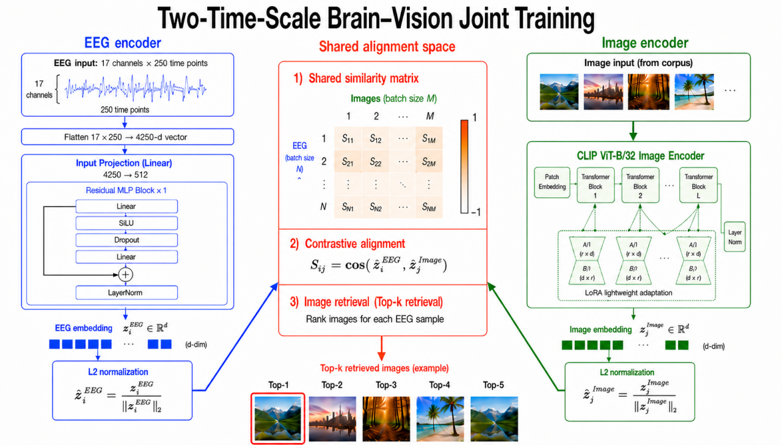
\includegraphics[width=0.99\linewidth]{figures/fig_framework_details.png}
  \caption{Detailed architecture of our method. During training, a compact EEG encoder and image-side LoRA adapters map paired EEG trials and stimulus images into a shared CLIP-aligned space and are optimized with a contrastive loss. The EEG branch learns at a faster rate than the image branch. During inference, a query EEG embedding is compared with a precomputed image bank to produce an ordinary Top-1/Top-5 ranking.}
  \label{fig:framework}
\end{figure}

\subsection{EEG encoder}

The input uses 17 posterior channels and 250 time samples. We flatten the $17\times250$ response, project it to 512 dimensions, and apply one residual two-layer MLP block with SiLU activation and layer normalization. This intentionally compact architecture limits capacity relative to the image backbone. The output is L2-normalized as in Equation~\ref{eq:embeddings}. Because the strict A/B/C experiment in Section~\ref{sec:abc} uses this identical EEG architecture in all conditions, its differences cannot be attributed to replacing the EEG encoder.

\subsection{Conservative image-side LoRA adaptation}

The image branch starts from a pretrained CLIP ViT-B/32 image checkpoint. Original CLIP weights remain frozen, and LoRA adapters are inserted into linear modules. The reference setting uses rank $r=32$, scaling $\alpha=32$, zero dropout, and Gaussian adapter initialization. If $W_0$ is a frozen image-layer matrix, the adapted layer is
\begin{equation}
h'=W_0h+\frac{\alpha}{r}BAh,
\label{eq:lora}
\end{equation}
where $A$ and $B$ are trainable low-rank factors. Unlike frozen-target alignment, Equation~\ref{eq:lora} allows the image space to move toward EEG-relevant structure while retaining the pretrained backbone.

\subsection{Contrastive objective and asymmetric optimization}

For a minibatch of $N$ paired EEG--image examples, we minimize symmetric cross-entropy over the similarity matrix:
\begin{equation}
\mathcal{L}=\frac{1}{2N}\sum_{i=1}^{N}
\left[-\log\frac{e^{S_{ii}}}{\sum_j e^{S_{ij}}}
-\log\frac{e^{S_{ii}}}{\sum_j e^{S_{ji}}}\right].
\label{eq:loss}
\end{equation}
The reference EEG learning rate is $5\times10^{-4}$, whereas the image-adapter learning rate is $5\times10^{-5}$, a ratio of 10:1. Both branches receive gradients from Equation~\ref{eq:loss}, but their update magnitudes differ. This is the operational meaning of asynchronous or two-time-scale learning in our method; it is not alternating training and does not use a separate objective.

\subsection{Optional batch-level matching}
\label{sec:matching_method}

Given a complete score matrix, independent retrieval uses $\hat{t}_i=\arg\max_jS_{ij}$. Greedy one-to-one decoding processes high-confidence queries first and removes selected images. Hungarian decoding instead solves
\begin{equation}
\hat{\pi}=\arg\max_{\pi\in\mathrm{Perm}(N)}\sum_{i=1}^{N}S_{i,\pi(i)},
\label{eq:hungarian}
\end{equation}
for a square session, while rectangular matrices leave surplus rows or columns unmatched. Stable matching uses query-proposing Gale--Shapley preferences derived from $S$. Sinkhorn applies log-domain scaling to an entropy-regularized transport plan, followed by row-wise plan decoding. We use temperature $0.05$, at most 500 iterations, and a strict residual tolerance of $10^{-8}$.

These structured methods naturally yield one assignment per query rather than a ranked list. We consequently report their \emph{assignment accuracy}, matched/unmatched counts, and convergence diagnostics. Top-5 is reported only for independent retrieval.

\section{Experimental Protocol}
\label{sec:protocol}

\subsection{Dataset, splits, and metrics}

We use THINGS-EEG2~\citep{gifford2022things}, containing EEG responses to natural object images from ten subjects. Following the standard zero-shot split, training and test concepts are disjoint, and evaluation uses 200 unseen test images. We select 17 posterior channels. Training inputs average four trials; standard test inputs average 80 repeated trials. Subject-dependent experiments train one model per subject. Strict LOSO trains on nine subjects and evaluates the tenth, producing ten folds. Repeated-trial averaging improves signal-to-noise ratio and is explicitly distinguished from single-trial decoding.

The primary subject-dependent result averages seeds $\{42,43,44,45,46\}$. We report the mean and sample standard deviation of the five seed-level ten-subject macro means. LOSO and the focused formal confirmation use seed 42 and are labeled single-seed. Random Top-1 and Top-5 levels in a 200-image gallery are $0.5\%$ and $2.5\%$, respectively.

\subsection{Optimization and checkpoint rules}

The reference model uses AdamW, cosine learning-rate decay, weight decay $0.05$, batch size 512, evaluation batch size 100, 25 epochs, bfloat16, gradient checkpointing, and a gradient-norm limit of 1.0 applied after back-propagation. The main historical grid uses the fixed final epoch to avoid selecting on test data. For fairness-suite NICE and ATM-S re-evaluations, one training run is performed and the checkpoint is selected by validation loss. Our method's fairness matrix reuses its fixed final checkpoint. We report these differences because the suite is a controlled implementation comparison, not a claim of perfect reproduction.

\subsection{Non-bijective robustness scenarios}

Matching assumptions are tested on identical scores under: the standard $200\times200$ session; removal of 5 or 10 EEG queries; removal of 5 or 10 images; asymmetric removal of both sides; duplication of 10 or 20 gallery images; addition of unrelated distractor images; addition of EEG queries whose correct image is absent; and combinations of missing, duplicated, and distractor items.

For a realistic duplicate-EEG condition, we do not copy score rows. Within every recording session, the first ten trials for an image are averaged into EEG-A-1 and the remaining ten into EEG-A-2. The two averages are disjoint real measurements. The base uses 200 EEG-A-1 queries; adding EEG-A-2 for 10 or 20 selected images produces $210\times200$ and $220\times200$ matrices. Their absolute scores are compared only within this 20-trial-average suite, not against the standard 80-trial test.

\section{Results}
\label{sec:results}

\subsection{Subject-dependent and cross-subject retrieval}

Table~\ref{tab:subject_results} follows the requested per-subject format. Literature rows use reported values under closely related 200-way THINGS-EEG2 protocols; encoder, preprocessing, checkpoint, and seed details still differ, so the table is contextual rather than a fully controlled ranking. Our subject-dependent row is the five-seed mean. Our LOSO row is a strict seed-42 re-evaluation and is marked accordingly.

\begin{table*}[t]
\centering
\caption{Per-subject 200-way EEG-to-image retrieval accuracy (\%). Intra trains and tests within one subject; Inter uses leave-one-subject-out evaluation. Published comparison rows are contextual. Our intra-subject values average five seeds; our inter-subject values are strict seed-42 LOSO (\textsuperscript{$\dagger$}).}
\label{tab:subject_results}
\setlength{\tabcolsep}{2.2pt}
\resizebox{\textwidth}{!}{%
\begin{tabular}{llrrrrrrrrrrr}
\toprule
Method & Metric & Sub1 & Sub2 & Sub3 & Sub4 & Sub5 & Sub6 & Sub7 & Sub8 & Sub9 & Sub10 & Avg. \\
\midrule
\multicolumn{13}{c}{\textit{Intra-subject: train and test on the same subject}} \\
\midrule
NICE~\citep{song2024nice} & Top-1 & 13.2&13.5&14.5&20.6&10.1&16.5&17.0&22.9&15.4&17.4&16.1\\
 & Top-5 &39.5&40.3&42.7&52.7&31.5&44.0&42.1&56.1&41.6&45.8&43.6\\
ATM-S~\citep{li2024visual} & Top-1 &25.6&22.0&25.0&31.4&12.9&21.3&30.5&38.8&34.4&29.1&27.1\\
 & Top-5 &60.4&54.5&62.4&60.9&43.0&51.1&61.5&72.0&51.5&63.5&58.1\\
UBP~\citep{wu2025ubp} & Top-1 &41.2&51.2&51.2&51.1&42.2&57.5&49.0&58.6&45.1&61.5&50.9\\
 & Top-5 &70.5&80.9&82.0&76.9&72.8&83.5&79.9&85.8&76.2&88.2&79.7\\
NeuroBridge~\citep{zhang2026neurobridge} & Top-1 &50.0&63.2&61.6&61.4&54.8&69.7&62.7&71.2&64.0&73.6&63.2\\
 & Top-5 &77.6&90.6&91.1&90.0&85.0&92.9&88.8&95.1&91.0&97.1&89.9\\
Shallow~\citep{du2026shallow} & Top-1 &75.4&87.3&82.9&79.1&74.9&90.2&79.0&86.9&81.3&89.3&82.6\\
 & Top-5 &94.3&99.0&\textbf{98.3}&\textbf{96.5}&96.4&99.2&97.3&99.4&\textbf{97.8}&99.2&97.7\\
\textbf{Our method} & \textbf{Top-1} &\textbf{84.0}&\textbf{89.7}&\textbf{85.2}&\textbf{83.4}&\textbf{84.0}&\textbf{92.8}&\textbf{84.8}&\textbf{90.9}&\textbf{80.3}&\textbf{91.5}&\textbf{86.66}\\
 & \textbf{Top-5} &\textbf{96.6}&\textbf{99.7}&97.4&\textbf{96.5}&\textbf{98.3}&\textbf{99.8}&\textbf{98.0}&\textbf{99.9}&97.7&\textbf{99.9}&\textbf{98.38}\\
\midrule
\multicolumn{13}{c}{\textit{Inter-subject: leave one subject out for test}} \\
\midrule
NICE~\citep{song2024nice} & Top-1 &7.6&5.9&6.0&6.3&4.4&5.6&5.6&6.3&5.7&8.4&6.2\\
 & Top-5 &22.8&20.5&22.3&20.7&18.3&22.2&19.7&22.0&17.6&28.3&21.4\\
ATM-S~\citep{li2024visual} & Top-1 &10.5&7.1&11.9&14.7&7.0&11.1&16.1&15.0&4.9&20.5&11.9\\
 & Top-5 &26.8&24.8&33.8&39.4&23.9&35.8&43.5&40.3&22.7&46.5&33.8\\
UBP~\citep{wu2025ubp} & Top-1 &11.5&15.5&9.8&13.0&8.8&11.7&10.2&12.2&15.5&16.0&12.4\\
 & Top-5 &29.7&40.0&27.0&32.3&33.8&31.0&23.8&32.2&40.5&43.5&33.4\\
NeuroBridge~\citep{zhang2026neurobridge} & Top-1 &23.2&21.2&\textbf{13.2}&17.0&14.5&\textbf{25.0}&15.3&\textbf{20.1}&13.7&27.2&19.0\\
 & Top-5 &52.4&49.3&\textbf{36.5}&45.3&37.7&\textbf{55.0}&45.1&44.9&36.5&56.3&45.9\\
Shallow~\citep{du2026shallow} & Top-1 &24.6&31.3&11.4&19.9&\textbf{19.0}&24.1&\textbf{18.6}&17.6&\textbf{23.3}&\textbf{34.6}&\textbf{22.4}\\
 & Top-5 &54.7&61.5&31.1&48.8&\textbf{45.5}&49.8&\textbf{51.6}&\textbf{46.7}&\textbf{54.9}&63.2&\textbf{50.8}\\
\textbf{Our method}$^{\dagger}$ & \textbf{Top-1} &\textbf{27.0}&\textbf{31.5}&13.0&\textbf{20.5}&14.0&15.5&17.0&15.0&20.0&30.5&20.40\\
 & \textbf{Top-5} &\textbf{59.0}&\textbf{63.5}&34.0&\textbf{50.5}&37.5&47.5&43.5&42.5&50.5&\textbf{64.5}&49.30\\
\bottomrule
\end{tabular}}
\end{table*}

The five seed-level subject-dependent macro means range from $85.60\%$ to $87.35\%$ Top-1 and from $98.20\%$ to $98.55\%$ Top-5, yielding $86.66\pm0.69\%$ and $98.38\pm0.14\%$. Our method is numerically strongest among the displayed intra-subject rows, but protocol differences preclude an unqualified state-of-the-art claim. In strict LOSO, the macro mean drops to $20.40\pm6.91\%$ Top-1 and $49.30\pm10.47\%$ Top-5 across held-out subjects. Figure~\ref{fig:loso} shows that all folds remain above chance but vary strongly, confirming that subject shift is still a central limitation.

\begin{figure}[t]
  \centering
  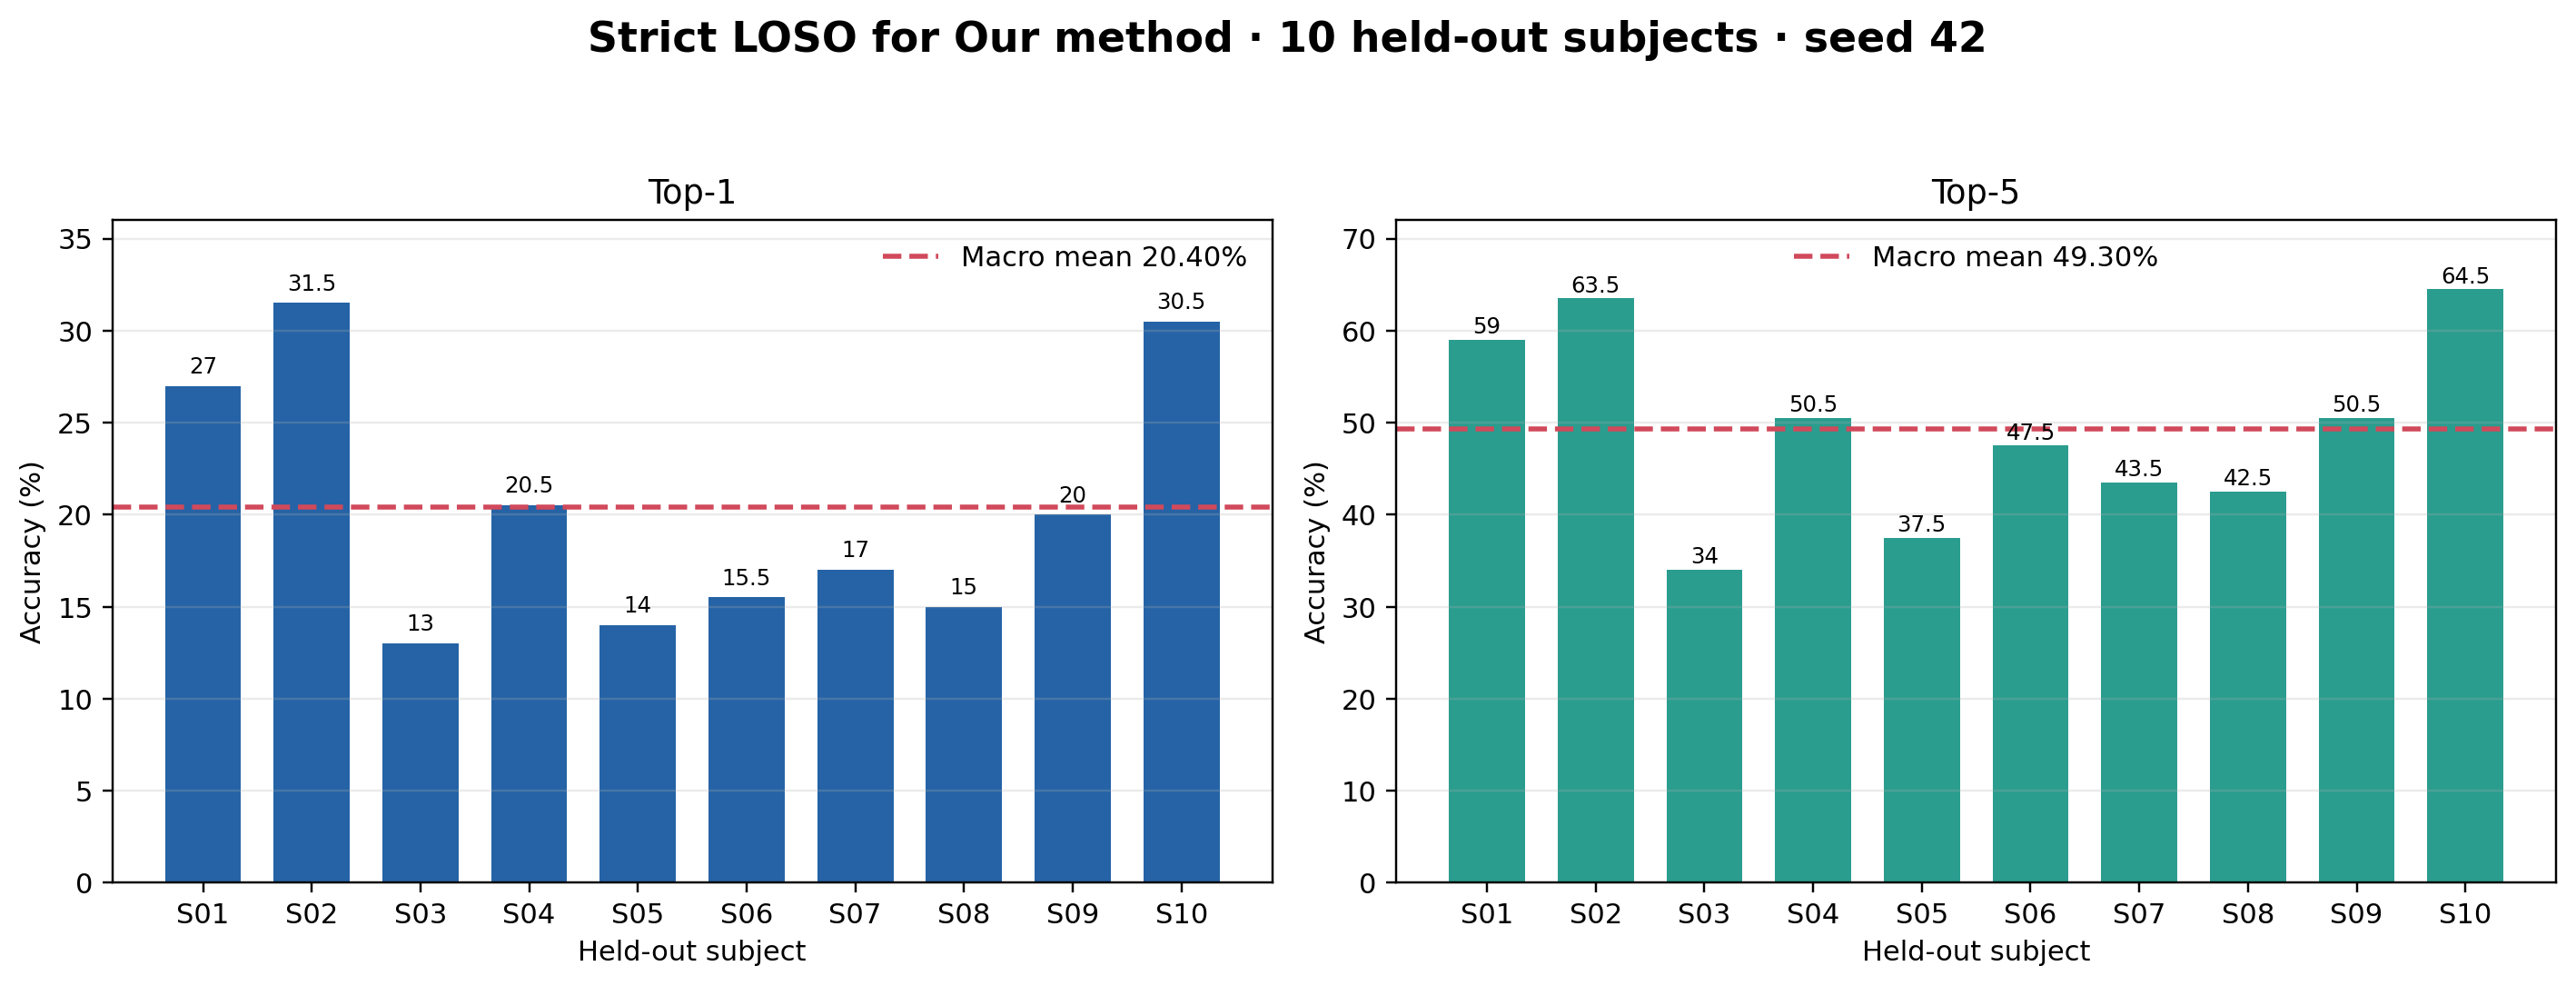
\includegraphics[width=0.88\linewidth]{figures/fig_loso_subjects.png}
  \caption{Strict leave-one-subject-out results at seed 42. Bars show independent-retrieval Top-1 and Top-5 for each held-out subject; dashed lines mark macro means. This is a single-seed generalization diagnostic rather than a five-seed population estimate.}
  \label{fig:loso}
\end{figure}

\subsection{Strict paired test of asymmetric co-adaptation}
\label{sec:abc}

The A/B/C experiment directly addresses whether the improvement is merely caused by our EEG encoder. All three settings use subject 08, seed 42, the same EEG encoder architecture and initialization, identical samples, objective, batch order, and training budget. Only image-side optimization differs. Figure~\ref{fig:ablation} shows that training the EEG encoder alone is insufficient: allowing image-side LoRA adaptation raises Top-1 by 32 points, and slowing the image update relative to the EEG update adds a further 27.5 points.

\begin{figure}[t]
  \centering
  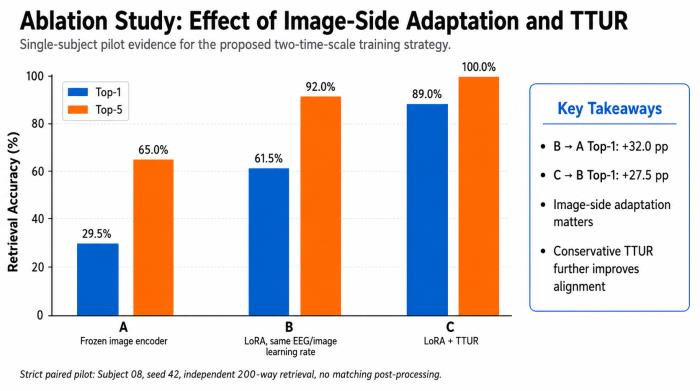
\includegraphics[width=0.78\linewidth]{figures/fig_ablation.png}
  \caption{Strict paired subject-08/seed-42 TTUR ablation. All arms use the identical EEG encoder: A freezes the image encoder, B adds equal-rate image-side LoRA, and C uses slower image-side LoRA updates. Values are independent-retrieval accuracy (\%).}
  \label{fig:ablation}
\end{figure}

Relative to A, C gains $+59.5$ Top-1 and $+35.0$ Top-5 points. Because the EEG architecture is controlled, the result supports our proposed innovation: high performance depends on dual-side co-adaptation and its asymmetric update schedule, not only on a newly chosen EEG encoder. It does not, by itself, prove that 10:1 is universally optimal; the next experiment examines nearby settings.

\subsection{Rank, learning-rate, and ratio study}

The focused validation grid crosses LoRA rank $r\in\{32,64\}$, EEG learning rate $\eta_e\in\{5\times10^{-4},10^{-3}\}$, and EEG-to-image learning-rate ratio $\rho\in\{5,10,20\}$, for 12 configurations on subject 08/seed 42. Table~\ref{tab:hparam_grid} reports validation scores. The highest validation Top-1 occurs at $(r,\eta_e,\rho)=(64,10^{-3},20)$.

\begin{table}[t]
\centering
\caption{Focused subject-08/seed-42 validation grid (\%). Image LR is $\eta_e/\rho$. Bold marks the best value in each metric; Top-1 determines the selected setting.}
\label{tab:hparam_grid}
\setlength{\tabcolsep}{5pt}
\begin{tabular}{rrrrr}
\toprule
Rank & EEG LR & Ratio & Top-1 & Top-5 \\
\midrule
32 & $5\times10^{-4}$ & 5  &31.03&59.94\\
32 & $5\times10^{-4}$ & 10 &31.52&60.24\\
32 & $5\times10^{-4}$ & 20 &29.52&57.64\\
32 & $10^{-3}$ & 5  &29.76&57.58\\
32 & $10^{-3}$ & 10 &33.76&62.91\\
32 & $10^{-3}$ & 20 &32.42&61.82\\
64 & $5\times10^{-4}$ & 5  &31.27&59.03\\
64 & $5\times10^{-4}$ & 10 &32.06&60.91\\
64 & $5\times10^{-4}$ & 20 &30.42&59.52\\
64 & $10^{-3}$ & 5  &27.39&55.88\\
64 & $10^{-3}$ & 10 &34.18&\textbf{63.33}\\
64 & $10^{-3}$ & 20 &\textbf{34.48}&63.03\\
\bottomrule
\end{tabular}
\end{table}

We then compare the selected configuration with the reference $(32,5\times10^{-4},10)$ across three subject-08 validation seeds and finally all ten subjects at seed 42. The selected validation mean is $34.44\%/63.74\%$ versus $31.23\%/60.97\%$ for the reference. In the formal paired test, Figure~\ref{fig:hparam} shows an average Top-1 increase from $85.85\%$ to $87.70\%$; Top-5 changes from $98.35\%$ to $98.30\%$. The selected setting wins Top-1 on eight of ten subjects, but it changes rank, absolute rate, and ratio jointly and uses one formal seed. The reference was protocol-locked before this focused study and is the only setting evaluated over all ten subjects and five seeds. We therefore do not retroactively replace the stronger-evidence headline with a post-hoc single-seed follow-up; the grid shows that asymmetric co-adaptation is robust to nearby choices, not that the original 10:1 ratio is globally optimal.

\begin{figure}[t]
  \centering
  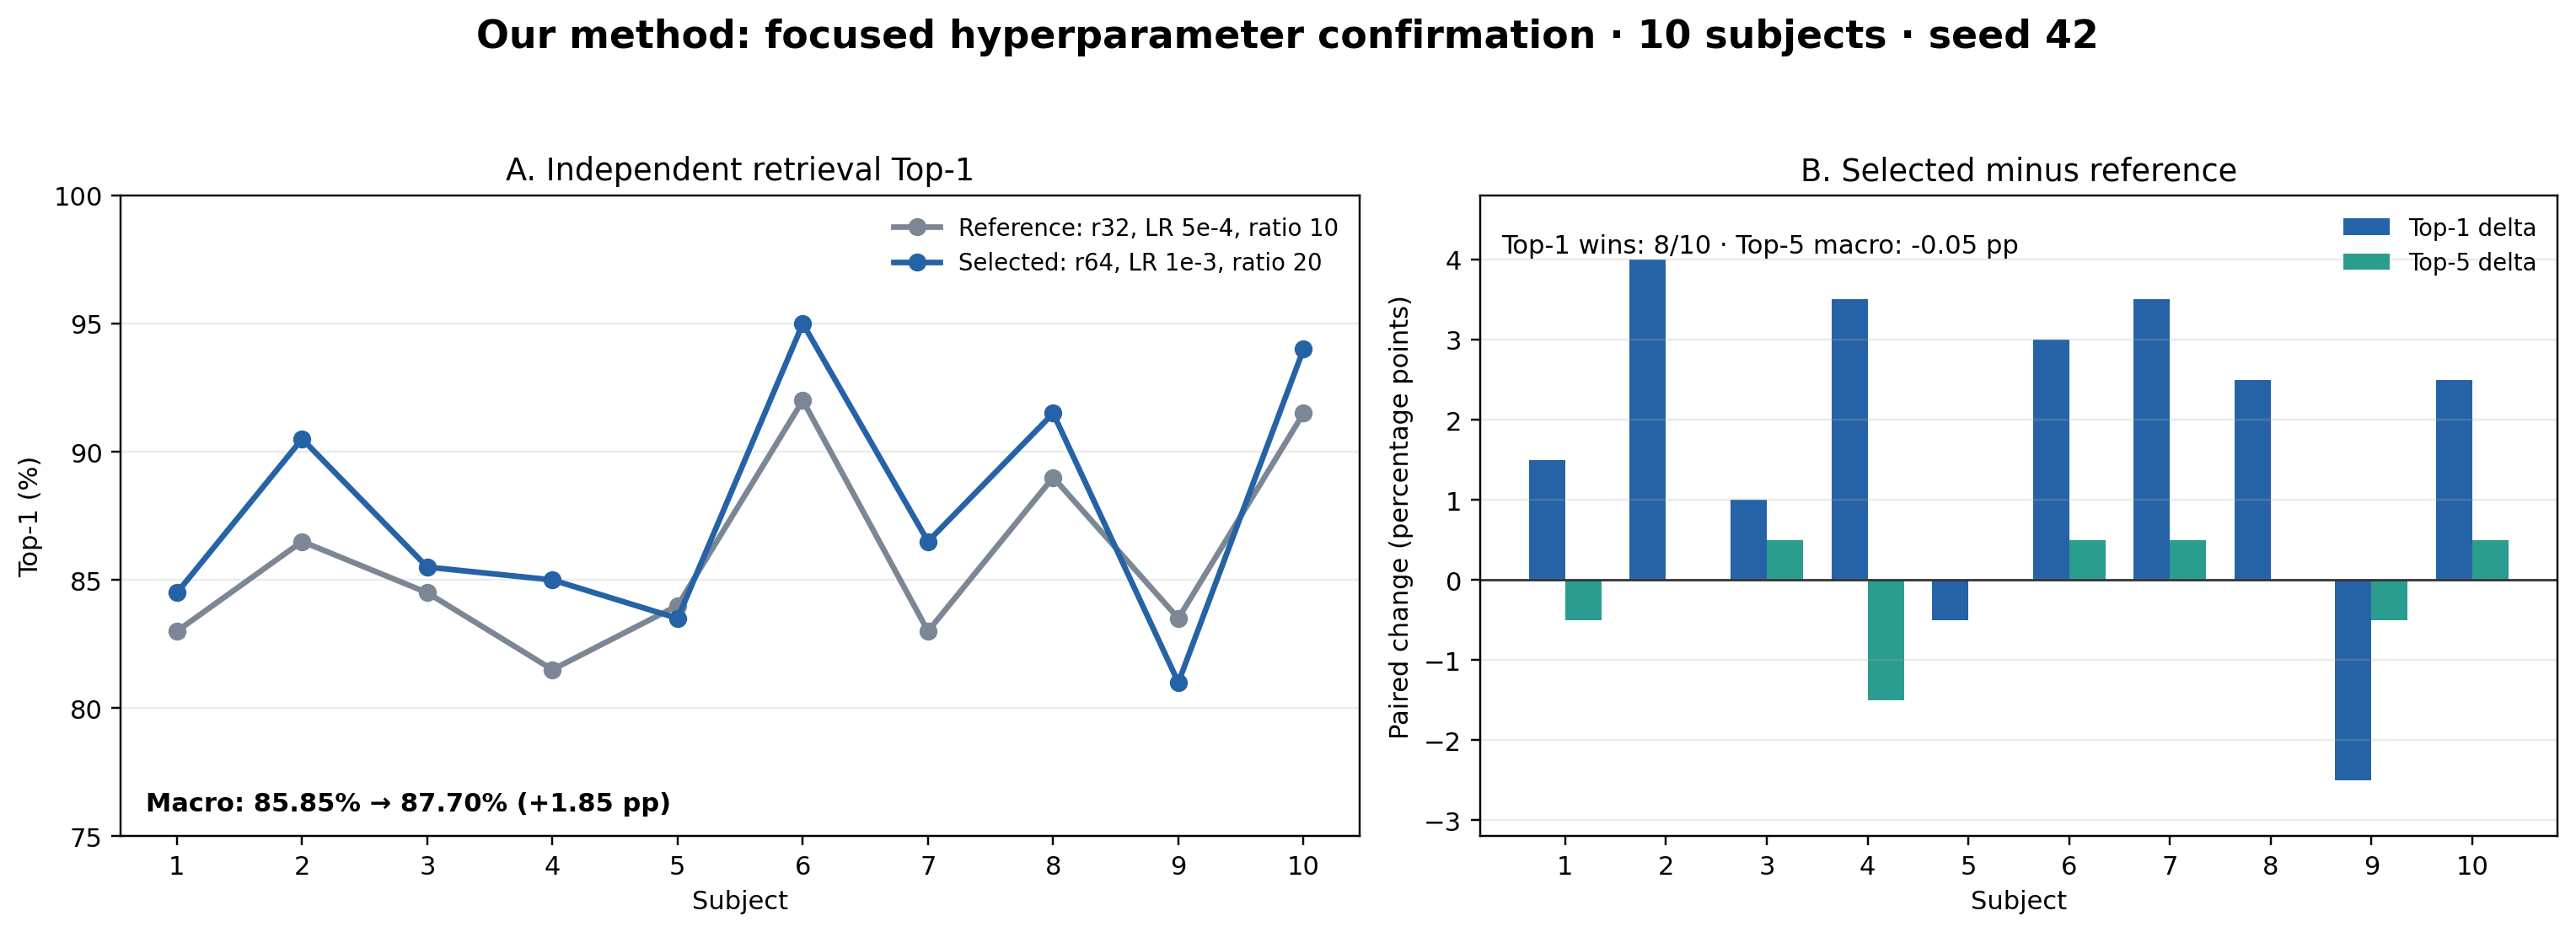
\includegraphics[width=0.90\linewidth]{figures/fig_hparam_confirmation.png}
  \caption{Formal ten-subject seed-42 confirmation of the validation-selected hyperparameter setting against the reference configuration. Top-1 improves by 1.85 points on average, while Top-5 is saturated and essentially unchanged.}
  \label{fig:hparam}
\end{figure}

\subsection{Fair comparison of matching algorithms}
\label{sec:matching_results}

We evaluate NICE, ATM-S, and our method on subject 08/seed 42. Within each baseline, all five decoders receive the exact same EEG queries, image gallery, labels, checkpoint, and score matrix. Thus only the matching rule changes. Table~\ref{tab:matching_standard} reports the standard $200\times200$ case. Independent Top-1/Top-5 remains the ordinary retrieval metric; the other columns are assignment accuracy.

\begin{table}[t]
\centering
\caption{Standard $200\times200$ fairness suite on subject 08/seed 42 (\%). Structured columns are assignment accuracy, not retrieval Top-1.}
\label{tab:matching_standard}
\resizebox{\linewidth}{!}{%
\begin{tabular}{lrrrrrr}
\toprule
Representation & Indep. T1 & Indep. T5 & Greedy & Hungarian & Stable & Sinkhorn$^{\ddagger}$ \\
\midrule
NICE &18.0&41.0&22.0&31.5&23.5&31.5\\
ATM-S &46.0&76.0&52.0&62.5&50.5&65.0\\
\textbf{Our method} &\textbf{91.0}&\textbf{99.5}&\textbf{95.5}&\textbf{100.0}&\textbf{98.0}&\textbf{100.0}\\
\bottomrule
\end{tabular}}
\vspace{2pt}

{\footnotesize $^{\ddagger}$Raw-score Sinkhorn did not meet the preregistered $10^{-8}$ tolerance within 500 iterations in these three cells; values are diagnostic.}
\end{table}

The standard session rewards hard global consistency: Hungarian increases assignment accuracy by 13.5, 16.5, and 9.0 points over independent Top-1 for NICE, ATM-S, and our method. This does not mean the representation improved. It means the decoder used the external fact that every query and image should appear exactly once. Applying the same decoder to every baseline makes the comparison fair, but the result remains an offline structured-assignment result.

The non-bijective suite in Figure~\ref{fig:matching_robustness} changes that conclusion. Removing only images creates unanswerable EEG queries; removing only EEG creates distractor gallery images; duplicate gallery entries create equivalent candidates; and combinations alter both matrix shape and answerability. The realistic disjoint-trial experiment is especially revealing. On the $200\times200$ 20-trial-average base, independent/Hungarian/Sinkhorn achieve $90.0/100.0/99.0\%$. At $210\times200$, they obtain $90.0/92.86/98.10\%$, with Hungarian leaving 10 queries unmatched. At $220\times200$, they obtain $90.45/89.09/96.36\%$, with Hungarian leaving 20 queries unmatched. The hard bijection is therefore beneficial only when its premise is true; multiple legitimate EEG queries per image turn it into a constraint violation.

\begin{figure}[t]
  \centering
  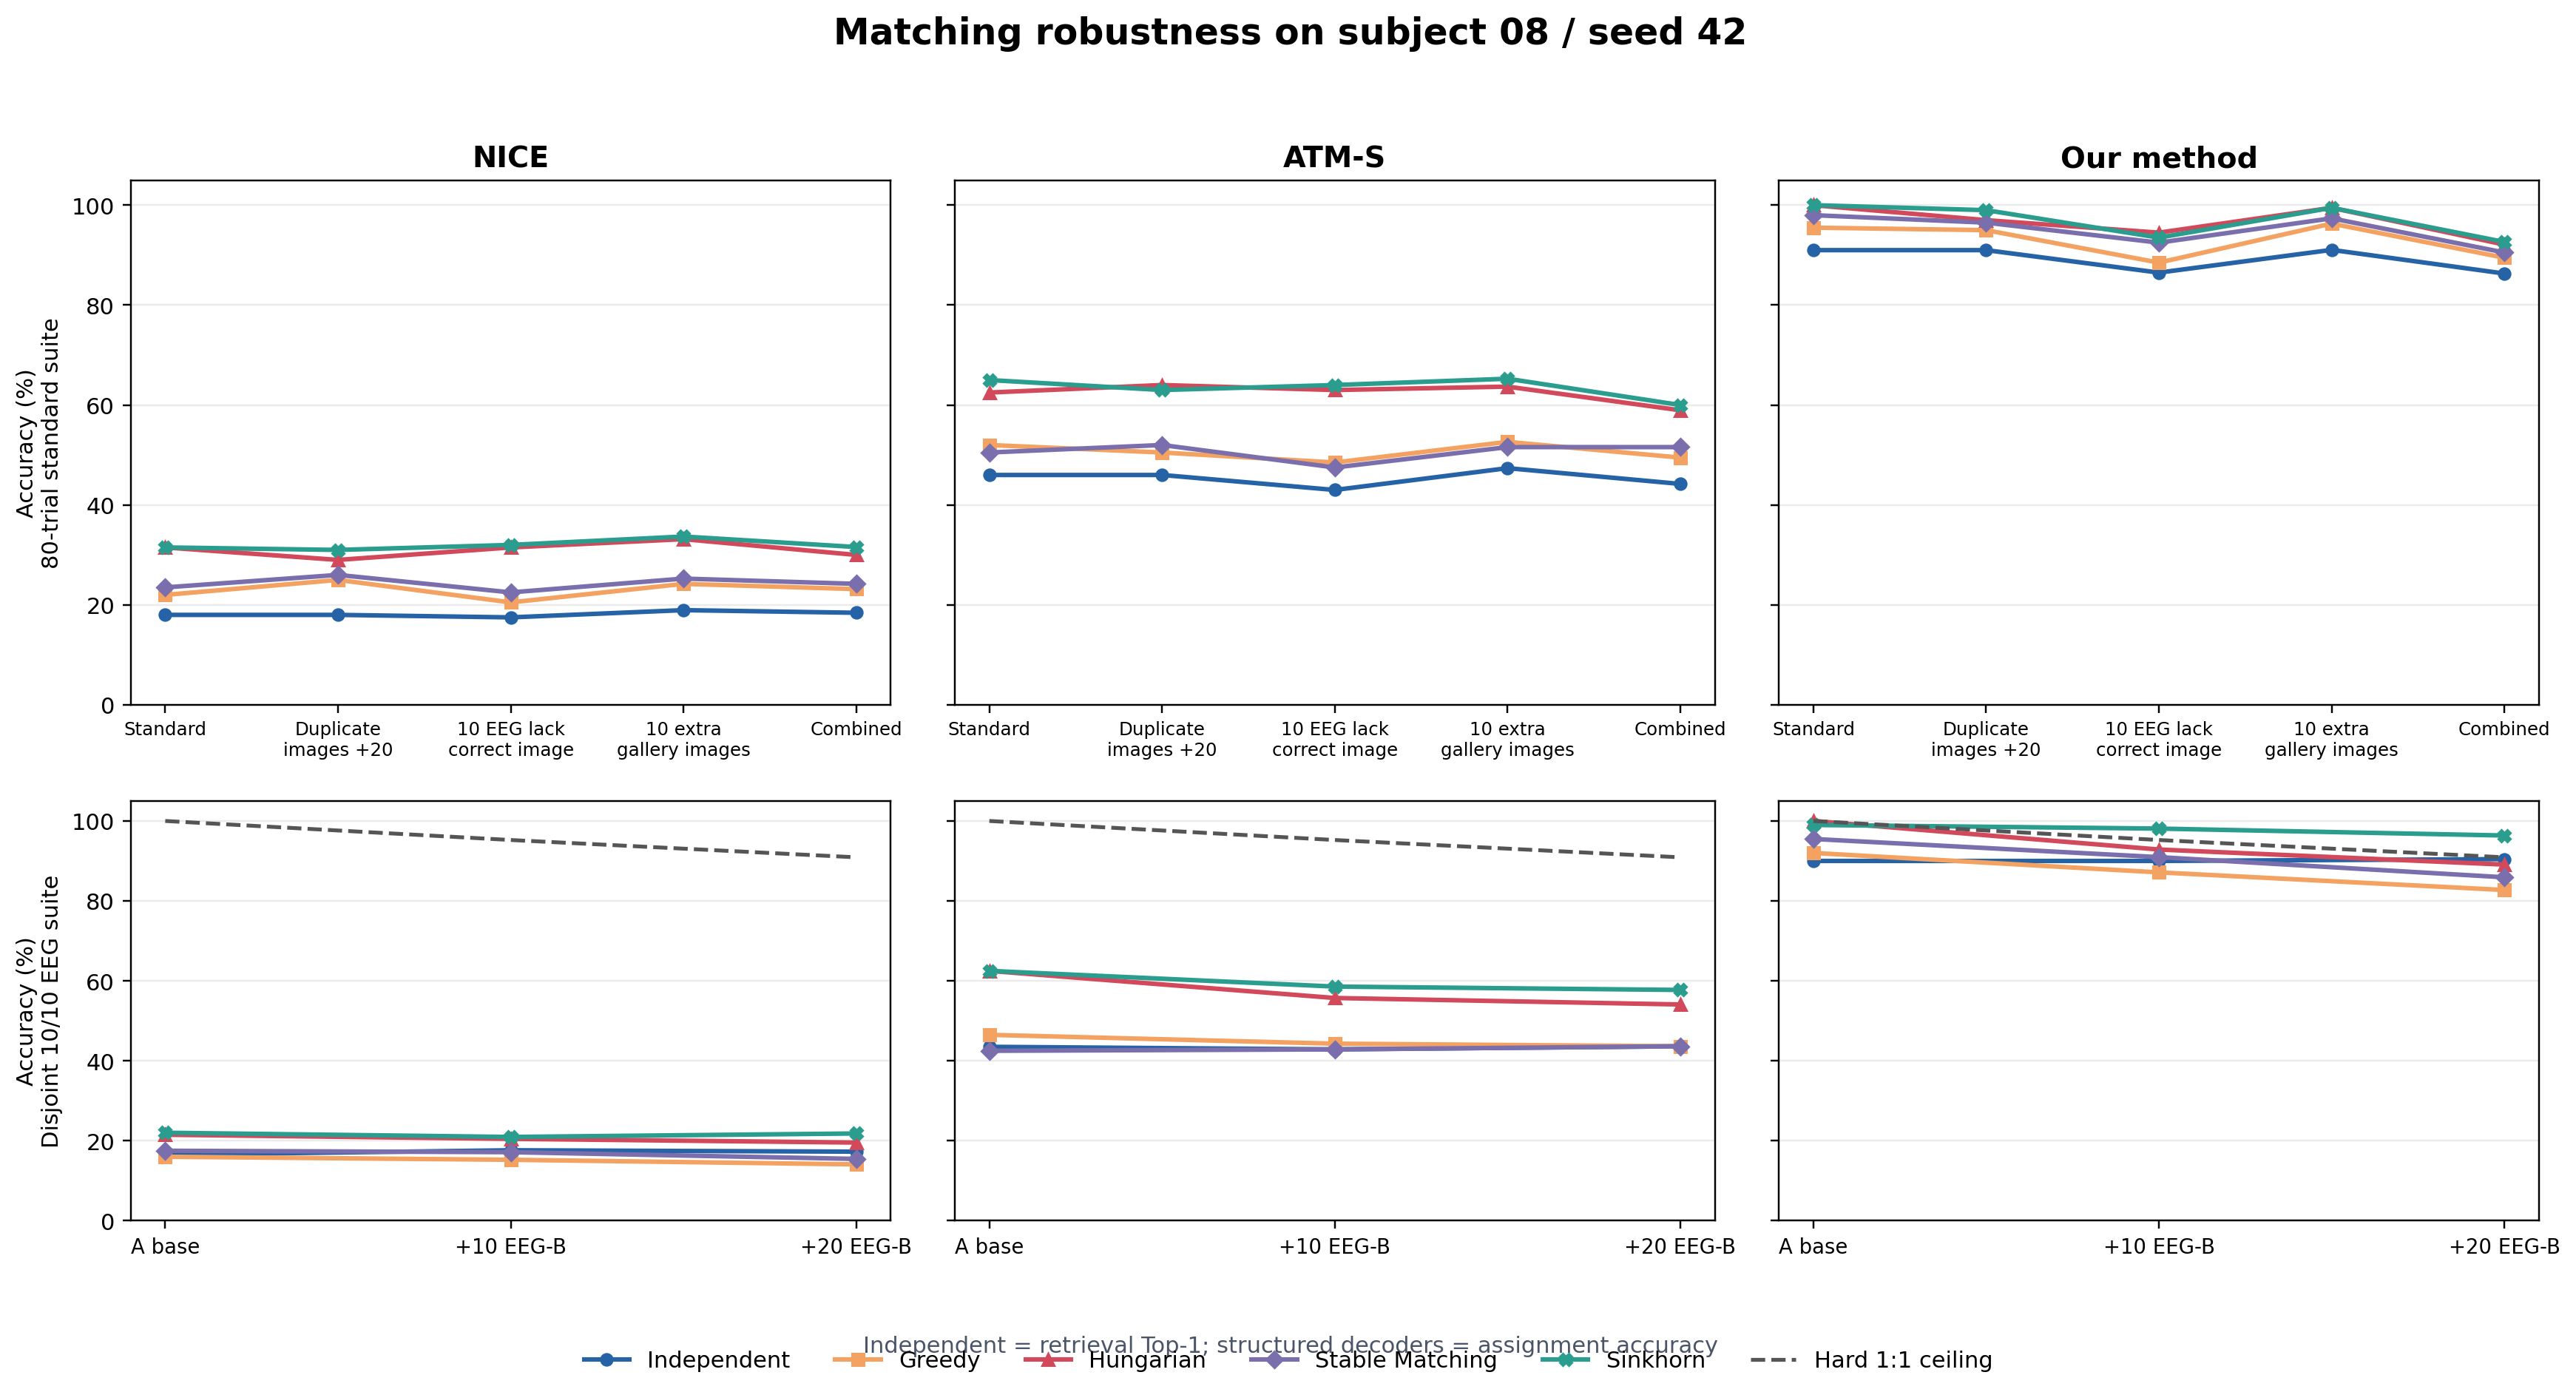
\includegraphics[width=0.92\linewidth]{figures/fig_matching_robustness.png}
  \caption{Matching robustness under missing, duplicate, and distractor items, including disjoint-trial duplicate EEG. Hard one-to-one assignment exposes unmatched queries when bijection is false.}
  \label{fig:matching_robustness}
\end{figure}

\subsection{Sinkhorn convergence audit}

Because Sinkhorn accuracy is meaningful only when its numerical behavior is known, we audit three score treatments over 90 cells each (three baselines by 30 scenarios): raw recorded scores; recorded-scale removal; and scale removal plus an epsilon schedule. Table~\ref{tab:sinkhorn} shows that scale removal greatly improves convergence but does not improve average assignment accuracy.

\begin{table}[t]
\centering
\caption{Sinkhorn audit over 90 baseline--scenario cells per setting.}
\label{tab:sinkhorn}
\begin{tabular}{lrrr}
\toprule
Score treatment & Conv. $10^{-6}$ & Conv. $10^{-8}$ & Mean assignment \\
\midrule
Raw recorded score & 30/90 & 25/90 & \textbf{62.83\%}\\
Recorded scale removed & 90/90 & 85/90 & 61.44\%\\
Scale removed + epsilon schedule & 90/90 & 85/90 & 61.44\%\\
\bottomrule
\end{tabular}
\end{table}

On the standard matrices, scale removal changes Sinkhorn assignment accuracy from $31.5\%$ to $33.0\%$ for NICE, from $65.0\%$ to $57.0\%$ for ATM-S, and leaves our method at $100.0\%$. The result rejects the simple hypothesis that better numerical convergence necessarily yields better matching. It also argues against spending the course-project budget on a learned matrix-transform network without a validation-defined objective and leakage-safe training split: convergence is a numerical property, whereas correct assignment depends on calibrated semantic structure.

\section{Discussion and Human-Centered Implications}
\label{sec:human}

\paragraph{What the system does and does not infer.}
Our evaluation decodes a stimulus from a known, closed 200-image gallery after repeated presentations. It is not open-world mind reading, does not reconstruct arbitrary thoughts, and does not establish semantic access beyond the experiment. Trial averaging uses substantial repeated evidence, so results should not be presented as single-glance decoding.

\paragraph{Privacy, consent, and agency.}
EEG is sensitive biometric and health-adjacent data. Deployment would require informed, revocable consent, purpose limitation, secure processing, restricted raw-signal retention, and clear uncertainty communication. Users should control calibration, deletion, and storage. This research system is not a medical device and should not support diagnosis, surveillance, employment screening, or covert inference.

\paragraph{Generalization and evaluation validity.}
The strict LOSO gap shows that cross-person transfer remains much weaker than subject-dependent calibration. Five seeds quantify optimization variability over the same stimuli, not new participants; literature rows also differ in encoders, preprocessing, and checkpoint rules. The subject-08 matching suite is diagnostic rather than population-level evidence, and batch matching can inflate apparent performance when a gallery is known to be a permutation. We therefore separate retrieval from assignment and test broken assumptions.

\paragraph{Technical limitations.}
Flattening discards explicit channel topology, and LoRA placement is not neurophysiologically targeted. The focused hyperparameter study is not a full factorial multi-seed search, while Sinkhorn row-wise decoding is a soft many-to-one diagnostic rather than a guaranteed discrete bijection. Future work should prioritize subject-invariant calibration, single-trial robustness, uncertainty, leakage-safe matcher calibration, and prospective studies of usefulness and trust.

\section{Conclusion}
\label{sec:conclusion}

Our asymmetric EEG--image co-adaptation reaches $86.66\%$ Top-1 and $98.38\%$ Top-5 over ten subjects and five seeds. With the EEG encoder fixed, the strict A/B/C ablation rises from $29.5\%$ to $61.5\%$ and $89.0\%$, isolating equal-rate and asymmetric image adaptation; focused tuning reaches $87.70\%$, while strict LOSO falls to $20.40\%$. Hungarian and Sinkhorn improve valid one-to-one assignments, not embeddings or standard Top-5, and weaken when correspondence fails.

\section*{Author contribution statement}
\label{sec:contributions}
{\small
\begin{itemize}[nosep,leftmargin=*]
  \item \textbf{Chi Kit Wong:} Overall brain--image co-adaptive framework and synchronized asymmetric joint optimization.
  \item \textbf{Sida Zhang:} Session-aware offline decoding as weighted bipartite matching; Hungarian/Sinkhorn analysis.
  \item \textbf{Zhiyi Chen:} Lightweight residual-MLP EEG representation module; hyperparameter analysis.
  \item \textbf{Ziyi Guo:} CLIP/LoRA image adaptation; conservative image-side learning rate.
\end{itemize}
\noindent\textbf{Equal contribution.} All members contributed equally to report writing, result interpretation, revision, and presentation preparation.
}

\paragraph{Generative-AI disclosure.}
OpenAI Codex assisted with code/log inspection, LaTeX/Markdown formatting, and language editing, including prompts to audit the page limit, reconcile saved CSV/JSON results, and repair equations. All outputs were reviewed and revised by the authors; drafts are retained in the project task history, and final claims remain the authors' responsibility.

\phantomsection
\label{sec:body_end}
\clearpage
\phantomsection
\label{sec:references}

\bibliographystyle{unsrtnat}
\bibliography{references}

\end{document}
